\documentclass[11pt,preprint, authoryear]{elsarticle}

\usepackage{lmodern}
%%%% My spacing
\usepackage{setspace}
\setstretch{1.2}
\DeclareMathSizes{12}{14}{10}{10}

% Wrap around which gives all figures included the [H] command, or places it "here". This can be tedious to code in Rmarkdown.
\usepackage{float}
\let\origfigure\figure
\let\endorigfigure\endfigure
\renewenvironment{figure}[1][2] {
    \expandafter\origfigure\expandafter[H]
} {
    \endorigfigure
}

\let\origtable\table
\let\endorigtable\endtable
\renewenvironment{table}[1][2] {
    \expandafter\origtable\expandafter[H]
} {
    \endorigtable
}


\usepackage{ifxetex,ifluatex}
\usepackage{fixltx2e} % provides \textsubscript
\ifnum 0\ifxetex 1\fi\ifluatex 1\fi=0 % if pdftex
  \usepackage[T1]{fontenc}
  \usepackage[utf8]{inputenc}
\else % if luatex or xelatex
  \ifxetex
    \usepackage{mathspec}
    \usepackage{xltxtra,xunicode}
  \else
    \usepackage{fontspec}
  \fi
  \defaultfontfeatures{Mapping=tex-text,Scale=MatchLowercase}
  \newcommand{\euro}{€}
\fi

\usepackage{amssymb, amsmath, amsthm, amsfonts}

\def\bibsection{\section*{References}} %%% Make "References" appear before bibliography


\usepackage[round]{natbib}

\usepackage{longtable}
\usepackage[margin=2.3cm,bottom=2cm,top=2.5cm, includefoot]{geometry}
\usepackage{fancyhdr}
\usepackage[bottom, hang, flushmargin]{footmisc}
\usepackage{graphicx}
\numberwithin{equation}{section}
\numberwithin{figure}{section}
\numberwithin{table}{section}
\setlength{\parindent}{0cm}
\setlength{\parskip}{1.3ex plus 0.5ex minus 0.3ex}
\usepackage{textcomp}
\renewcommand{\headrulewidth}{0.2pt}
\renewcommand{\footrulewidth}{0.3pt}

\usepackage{array}
\newcolumntype{x}[1]{>{\centering\arraybackslash\hspace{0pt}}p{#1}}

%%%%  Remove the "preprint submitted to" part. Don't worry about this either, it just looks better without it:
\makeatletter
\def\ps@pprintTitle{%
  \let\@oddhead\@empty
  \let\@evenhead\@empty
  \let\@oddfoot\@empty
  \let\@evenfoot\@oddfoot
}
\makeatother

 \def\tightlist{} % This allows for subbullets!

\usepackage{hyperref}
\hypersetup{breaklinks=true,
            bookmarks=true,
            colorlinks=true,
            citecolor=blue,
            urlcolor=blue,
            linkcolor=blue,
            pdfborder={0 0 0}}


% The following packages allow huxtable to work:
\usepackage{siunitx}
\usepackage{multirow}
\usepackage{hhline}
\usepackage{calc}
\usepackage{tabularx}
\usepackage{booktabs}
\usepackage{caption}


\newenvironment{columns}[1][]{}{}

\newenvironment{column}[1]{\begin{minipage}{#1}\ignorespaces}{%
\end{minipage}
\ifhmode\unskip\fi
\aftergroup\useignorespacesandallpars}

\def\useignorespacesandallpars#1\ignorespaces\fi{%
#1\fi\ignorespacesandallpars}

\makeatletter
\def\ignorespacesandallpars{%
  \@ifnextchar\par
    {\expandafter\ignorespacesandallpars\@gobble}%
    {}%
}
\makeatother

\newenvironment{CSLReferences}[2]{%
}

\urlstyle{same}  % don't use monospace font for urls
\setlength{\parindent}{0pt}
\setlength{\parskip}{6pt plus 2pt minus 1pt}
\setlength{\emergencystretch}{3em}  % prevent overfull lines
\setcounter{secnumdepth}{5}

%%% Use protect on footnotes to avoid problems with footnotes in titles
\let\rmarkdownfootnote\footnote%
\def\footnote{\protect\rmarkdownfootnote}
\IfFileExists{upquote.sty}{\usepackage{upquote}}{}

%%% Include extra packages specified by user

%%% Hard setting column skips for reports - this ensures greater consistency and control over the length settings in the document.
%% page layout
%% paragraphs
\setlength{\baselineskip}{12pt plus 0pt minus 0pt}
\setlength{\parskip}{12pt plus 0pt minus 0pt}
\setlength{\parindent}{0pt plus 0pt minus 0pt}
%% floats
\setlength{\floatsep}{12pt plus 0 pt minus 0pt}
\setlength{\textfloatsep}{20pt plus 0pt minus 0pt}
\setlength{\intextsep}{14pt plus 0pt minus 0pt}
\setlength{\dbltextfloatsep}{20pt plus 0pt minus 0pt}
\setlength{\dblfloatsep}{14pt plus 0pt minus 0pt}
%% maths
\setlength{\abovedisplayskip}{12pt plus 0pt minus 0pt}
\setlength{\belowdisplayskip}{12pt plus 0pt minus 0pt}
%% lists
\setlength{\topsep}{10pt plus 0pt minus 0pt}
\setlength{\partopsep}{3pt plus 0pt minus 0pt}
\setlength{\itemsep}{5pt plus 0pt minus 0pt}
\setlength{\labelsep}{8mm plus 0mm minus 0mm}
\setlength{\parsep}{\the\parskip}
\setlength{\listparindent}{\the\parindent}
%% verbatim
\setlength{\fboxsep}{5pt plus 0pt minus 0pt}



\begin{document}



\begin{frontmatter}  %

\title{22581340\_Netflix}

% Set to FALSE if wanting to remove title (for submission)




\author[Add1]{Gabriella Neilon}
\ead{22581340@sun.ac.za}





\address[Add1]{Stellenbosch University}

\cortext[cor]{Corresponding author: Gabriella Neilon}

\begin{abstract}
\small{
This report delves into several key aspects of the film industry,
including the dominant genre, country, source of entertainment, dominant
actors and directors, as well as a movie recommendation generator based
on these specifications. By analyzing these elements, I uncover the
prevalent genres and countries in the industry to identifying
influential actors and directors. Furthermore, the movie recommendation
generator serves as a practical tool for personalised film suggestions,
taking into account specific preferences and criteria.
}
\end{abstract}

\vspace{1cm}





\vspace{0.5cm}

\end{frontmatter}

\setcounter{footnote}{0}



%________________________
% Header and Footers
%%%%%%%%%%%%%%%%%%%%%%%%%%%%%%%%%
\pagestyle{fancy}
\chead{}
\rhead{}
\lfoot{}
\rfoot{\footnotesize Page \thepage}
\lhead{}
%\rfoot{\footnotesize Page \thepage } % "e.g. Page 2"
\cfoot{}

%\setlength\headheight{30pt}
%%%%%%%%%%%%%%%%%%%%%%%%%%%%%%%%%
%________________________

\headsep 35pt % So that header does not go over title




\hypertarget{introduction}{%
\section{\texorpdfstring{Introduction
\label{Introduction}}{Introduction }}\label{introduction}}

In this comprehensive report, I delve into various aspects of the movie
industry, exploring genres, entertainment types, dominant countries,
influential actors and directors, and even a movie generation
recommender. Through meticulous analysis and visualization, I aim to
provide insights into the fascinating world of movies, shedding light on
trends, preferences, and recommendations. From examining popular genres
to uncovering dominant production countries, this report offers a
diverse perspective on the cinematic landscape.

\hypertarget{part-a}{%
\section{Part A}\label{part-a}}

In this section I explore the most popular genres. Trends in Netflix
content

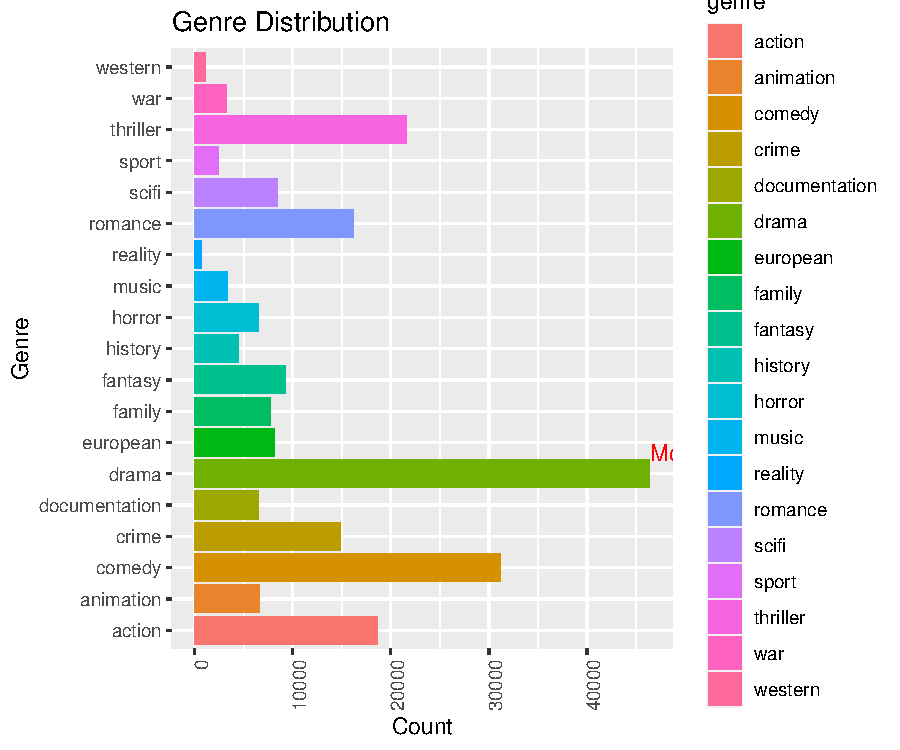
\includegraphics{Question4_files/figure-latex/unnamed-chunk-1-1.pdf}

Based on the graph presented above, it is evident that the most popular
genre among the analyzed movies is drama, followed by comedy and
thriller. On the other hand, the least popular genre appears to be
western. These findings shed light on the preferences of viewers,
highlighting the widespread appeal of emotionally engaging narratives
and the enduring popularity of comedic and suspenseful storytelling.

Moving forward, let's delve into the analysis of entertainment types to
determine whether movies or shows hold greater popularity among
audiences.

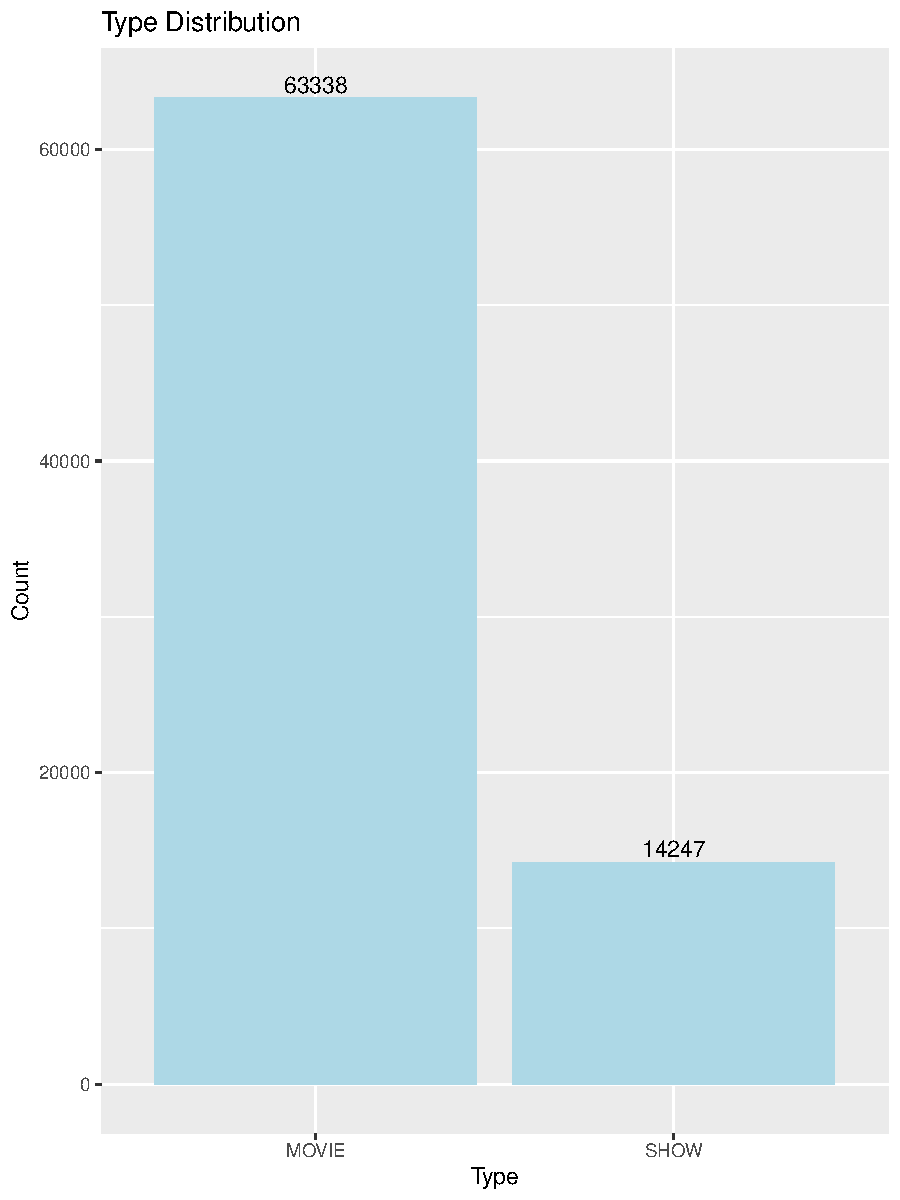
\includegraphics{Question4_files/figure-latex/unnamed-chunk-2-1.pdf}

The graph clearly illustrates that movies enjoy a higher level of
popularity compared to shows. This finding indicates that audiences have
a stronger preference for movies as their preferred form of
entertainment.

\hypertarget{country-wide-analysis}{%
\section{Country-wide Analysis}\label{country-wide-analysis}}

In this section, I present a visual representation of the top 10
countries in terms of dominant movie productions. By mapping these
countries, we can gain valuable insights into the global landscape of
the film industry and identify the key players in movie production.

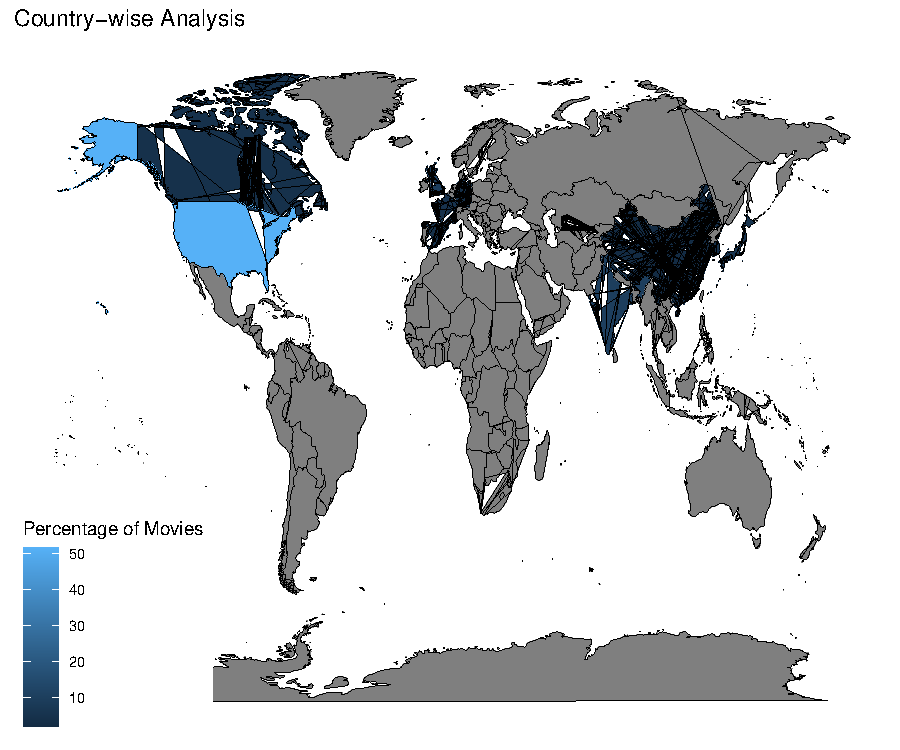
\includegraphics{Question4_files/figure-latex/unnamed-chunk-3-1.pdf}

\hypertarget{dominant-actors-and-directors}{%
\section{Dominant actors and
directors}\label{dominant-actors-and-directors}}

In this section, I delve into the world of cinema to identify the top
actors and directors per country and genre, based on their IMDb scores.
By analyzing the IMDb scores, which serve as a measure of critical
acclaim and audience appreciation, we can determine the leading talents
in the film industry across different countries and genres. This
exploration allows us to highlight the exceptional performances and
directorial prowess that have garnered recognition and acclaim within
their respective fields.

\begin{table}
\begin{table}

\caption{\label{tab:unnamed-chunk-4}Dominant Actors}
\centering
\begin{tabular}[t]{l|l|l}
\hline
Country Code & Dominating Actor & Dominating Genre\\
\hline
ca & Ben Browder & scifi\\
\hline
cn & Benedict Lim & documentation\\
\hline
de & Keanu Reeves & horror\\
\hline
es & Caterina Murino & drama\\
\hline
fr & Michael Peterson & crime\\
\hline
gb & Leonardo DiCaprio & scifi\\
\hline
in & Darsheel Safary & family\\
\hline
jp & Koichi Yamadera & western\\
\hline
us & Jerry Seinfeld & comedy\\
\hline
\end{tabular}
\end{table}\begin{table}

\caption{\label{tab:unnamed-chunk-4}Dominant Directors}
\centering
\begin{tabular}[t]{l|l|l}
\hline
Country Code & Dominating Director & Dominating Genre\\
\hline
ca & Ben Browder & scifi\\
\hline
cn & Benedict Lim & documentation\\
\hline
de & Keanu Reeves & horror\\
\hline
es & Caterina Murino & drama\\
\hline
fr & Michael Peterson & crime\\
\hline
gb & Leonardo DiCaprio & scifi\\
\hline
in & Darsheel Safary & family\\
\hline
jp & Koichi Yamadera & western\\
\hline
us & Jerry Seinfeld & comedy\\
\hline
\end{tabular}
\end{table}
\end{table}

\hypertarget{movie-recommendation}{%
\section{Movie recommendation}\label{movie-recommendation}}

For an entertaining twist, I have developed a movie generation
recommender based on the exploratory analysis conducted. Specifically, I
focused on a combination of criteria, including the name ``Caterina
Murino,'' production countries limited to the United States, a minimum
IMDb score of 8, and the genre specified as drama. By leveraging these
parameters, the recommender system suggests movies that align with these
specific preferences.

\begin{verbatim}
## [1] "365 Days: This Day"
\end{verbatim}

\hfill

\hypertarget{conclusion}{%
\section{Conclusion}\label{conclusion}}

In conclusion, this report has taken us on a captivating journey through
the realm of movies. We have witnessed the popularity of different
genres, with drama, comedy, and thriller taking the lead. The
exploration of entertainment types revealed movies to be the favored
choice among audiences. By mapping dominant movie production countries,
we gained a deeper understanding of the global nature of the film
industry. Additionally, identifying top actors and directors based on
IMDb scores showcased the talent and influence of these individuals
across countries and genres.

To add an extra touch of enjoyment, I even developed a movie generation
recommender, tailored to specific criteria, such as the name of an
actress, desired production countries, IMDb score, and preferred genre.
This tool serves as a fun way to discover captivating films that meet
your specific preferences.

\bibliography{Tex/ref}





\end{document}
